\section{Evaluation} \label{eval}

In this chapter, we present our evaluation procedure, which we use to assess the performance of the approaches. We have created three evaluation sets with the metadata from the repositories. Two of them consider only fields, whereas the third one considers all subjects. We evaluate the approaches on these sets with two different metrics, one that measures the hit rate of the assignments and one that uses the hierarchy to evaluate if the guesses are close to the correct subject. 

We discard performing a survey because every sample would require cross-checking, as human judges are inconsistent \cite{csomai2007investigations}. Furthermore, given how technical our documents are, assessing the appropriateness of a subject assignment might prove difficult for someone who is not well-read in the topics of the document. Another disadvantage is that numerous assignments have to be evaluated for the survey to gain statistical significance. Thus, we would need to gather experts in various fields (multiple per field) and have them assess many assignments. We therefore leave the survey for future work.

As we discussed when analyzing the repositories (section \ref{repo_analysis_subjects}), most of the popular subjects in the repositories are \acrfull{ddc} subjects. These are usually broader in their meaning, but are still useful descriptors of the topics handled by a document. We present how we have incorporated them into our evaluation procedure in section \ref{eval_ddc}. Essentially, given that we have to manually assign them to \acrshort{mag} subjects, we have mapped them to the fields. They will therefore be useful to evaluate if the indexing methods have grasped the broad meaning of the documents.

Venues, advisors and referees also describe the content of the documents they are assigned to. We therefore create another evaluation set with them. As for the \acrshort{ddc} evaluation set, in section \ref{eval_venues} we map popular venues, advisors and referees manually to the fields of study, and then retrieve their associated documents.

We create our final evaluation set by automatically mapping subjects present in the repositories to the ones in our subset of \acrshort{mag} subjects. This evaluation set is the only one that considers subjects that are not fields, and is thus the one that determines is the approach is able to correctly model the 2,157 labels we consider in this thesis.

We measure the performance of the models on these evaluation sets with two different metrics. The first outputs one if the correct subject is included in the top $k$ subjects output by a model, and otherwise zero. The second one, given a subject and a candidate output by a model, outputs a value between zero and one that describes how close the candidate is to the subject in the hierarchy. We present both metrics in section \ref{eval_metrics}, as well as other metrics we have found in the literature.

After presenting the evaluation sets and metrics, we use them to compare the candidates of each approach and then compare the resulting models to one another. Interestingly, our evaluation procedure indicates that our own word embeddings yield better results in the unsupervised approach than pre-trained embeddings. Regarding the supervised approach, we find out that extending the model with asymmetry or coherence does not improve the performance of the model, which may be because some parameters were optimized for the initial model, without considering the two extensions. Still, the supervised approach yields the best results in all evaluation sets and for both metrics.

We end this chapter by analyzing the impact of representation length on the hit rate of the supervised model. We find out that the hit rate of the model for documents that are represented by less than 50 tokens is over 20 \% worse than for larger representations. This indicates that our results could be improved by adding missing abstracts, and fixing those that are in other languages.

\subsection{Evaluation sets} \label{eval_datasets}

Subject assignments can be evaluated with the metadata of the documents. \cite{toepfer2020fusion} mentions this possibility, stating that they plan on developing an automatic quality estimation metric that is based on meta information of the documents. For example, documents that are published in the same journal can be expected to be semantically similar. The publisher clearly delimits the field to which the publication belongs to. Our approach, although it also uses the metadata to evaluate the methods, is more straight forward. We extract subjects and venues (including referees and advisors of theses) from the repositories to construct three evaluation sets.

The first evaluation set comprises the handwritten subjects of the repositories, i.e. those that the users input manually when uploading a new document. We have mapped our complete set of subjects to the handwritten subjects of the repositories with a string matching procedure. Doing so, we could create an evaluation set with over 9,000 assignments. This evaluation set is the only one that considers further subjects, other than fields.

\acrshort{ddc} subjects can also be used in this regard. They appear consistently throughout all three repositories, as shown in section \ref{subjects_ddc}, and don't suffer from potential duplicates that arise from the free-text input, as handwritten subjects do. We have manually mapped \acrshort{ddc} numbers to \acrshort{mag} fields of study, to construct our second evaluation set.

Using unsupervised methods to evaluate the set of subjects of theses may prove more challenging, as they are not published anywhere and their authors usually just have that one document in the repositories. Advisors and referees may be of use in this regard. Two theses advised by the same professor should be more similar than two theses advised by different professors. This is the same logic we followed in the \acrfull{um}. We create our third evaluation set by manually mapping venues, advisors and referees to \acrshort{mag} fields of study.

\subsubsection{Handwritten subjects} \label{eval_subjects}

We have mapped our subset of \acrshort{mag} subjects to those of the repositories, which were input manually by the users that uploaded the documents, hence the term ``handwritten subjects''. To increase the number of matches, we have done so in a case-insensitive manner, i.e. we have first lower-cased all subjects. This simple matching procedure yielded 1,272 subjects, meaning that 59 \% of our \acrshort{mag} subset is present in the repositories. The total number of assignments of subjects to documents is 9,052.

The most popular subjects are \textit{Climate change}, which is assigned to 154 documents, \textit{Sustainability}, with 124 assignments, \textit{Mass spectrometry}, with 87 assignments and \textit{Molecular dynamics}, with 76 assignments. Figure \ref{fig:docs_per_subject} shows how often each subject occurs in the repositories. 301 subjects are assigned to only one document, whereas 307 subjects are assigned to at least nine documents. On average, the subjects are assigned to seven documents of the repositories.

\begin{figure}
  \begin{subfigure}[t]{0.45\textwidth}
    \centering
    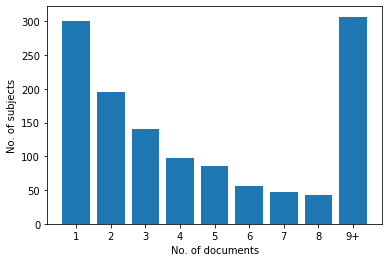
\includegraphics[width=\textwidth]{figures/evaluation/docs_per_subject.png}
    \caption{Handwritten subjects.}
    \label{fig:docs_per_subject}
  \end{subfigure}
  \hfill
  \begin{subfigure}[t]{0.45\textwidth}
    \centering
    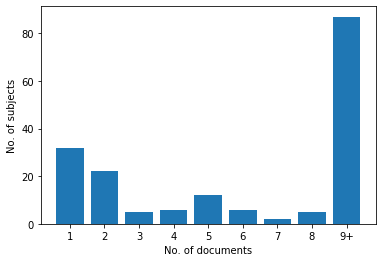
\includegraphics[width=\textwidth]{figures/evaluation/docs_per_ddc.png}
    \caption{DDC subjects.}
    \label{fig:docs_per_ddc}
  \end{subfigure}
  \caption{Distribution of the number of documents each subject (handwritten or DDC) is assigned to.}
\end{figure}

Another positive aspect of these subject matches is how well distributed they are across the fields. As can be seen in figure \ref{fig:eval_hw_fields}, all fields have assignments. \textit{Environmental science} is the least populated field, with 41 assignments. On the other hand, \textit{Medicine}, \textit{Biology} and \textit{Physics} have more than 200 assignments each.

\begin{figure}
  \begin{subfigure}[t]{\textwidth}
    \centering
    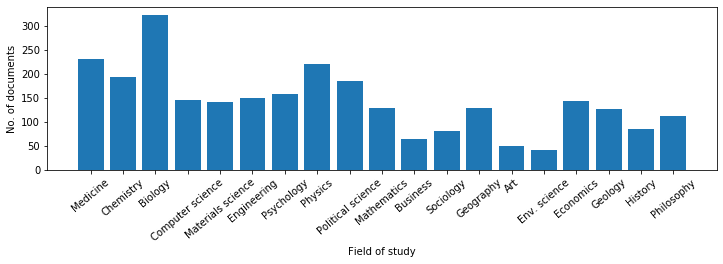
\includegraphics[width=\textwidth]{figures/evaluation/eval_hw_fields.png}
    \caption{Handwritten subjects}
    \label{fig:eval_hw_fields}
  \end{subfigure}
  \hfill
  \begin{subfigure}[t]{\textwidth}
    \centering
    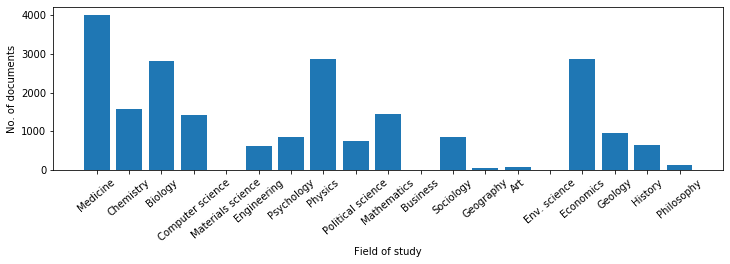
\includegraphics[width=\textwidth]{figures/evaluation/eval_ddc_fields.png}
    \caption{DDC subjects}
    \label{fig:eval_ddc_fields}
  \end{subfigure}
  \begin{subfigure}[t]{\textwidth}
    \centering
    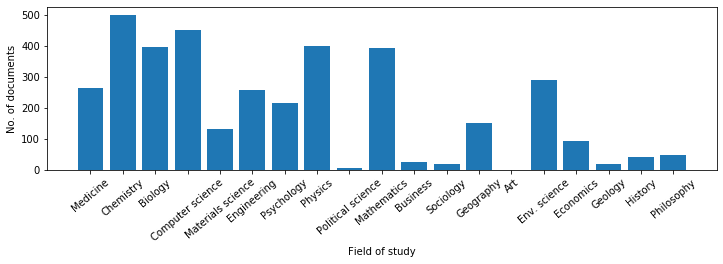
\includegraphics[width=\textwidth]{figures/evaluation/eval_venue_fields.png}
    \caption{Venues}
    \label{fig:eval_venue_fields}
  \end{subfigure}
  \caption{Number of assignments per field of study for handwritten subjects, DDC subjects and venues.}
\end{figure}

This evaluation set comprises 7,145 distinct documents. 78 \% of them only have one of the \acrshort{mag} subjects assigned to them, as shown in figure \ref{fig:eval_hw_fields}. On average, documents are assigned 1.27 subjects. Only one document has more than six assignments. It belongs to edoc and its subjects include \textit{Sustainability}, \textit{Climate change} and \textit{Poverty}, among others. Then there are two documents of refubium with six assignments, one about public law and the other about magnesium, potassium and other chemical elements.

The documents are also evenly distributed across repositories. Refubium has the largest amount of documents in this evaluation set, with 3,208. This makes sense, given that it contains 47 \% of all the documents in our dataset. Depositonce has 2,192 documents and edoc, 1,745. As percentages of their total number of documents, all repositories have more than 20 \% of their documents in this evaluation set. Depositonce leads the way with 29 \%, followed by edoc, with 23 \%, and refubium, with 22 \%.

\begin{figure}
  \begin{subfigure}[t]{0.45\textwidth}
    \centering
    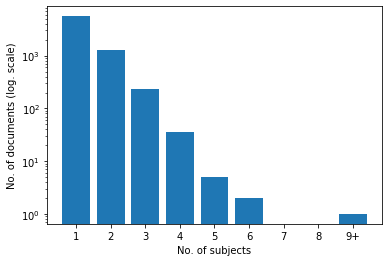
\includegraphics[width=\textwidth]{figures/evaluation/subjects_per_doc.png}
    \caption{Handwritten subjects.}
    \label{fig:subjects_per_doc}
  \end{subfigure}
  \hfill
  \begin{subfigure}[t]{0.45\textwidth}
    \centering
    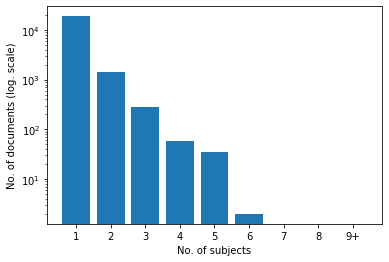
\includegraphics[width=\textwidth]{figures/evaluation/ddc_per_doc.png}
    \caption{DDC subjects.}
    \label{fig:ddc_per_doc}
  \end{subfigure}
  \caption{Number of subjects (handwritten or DDC) assigned to each document.}
\end{figure}

\subsubsection{DDC subjects} \label{eval_ddc}

Mapping \acrshort{ddc} subjects to \acrshort{mag} subjects was more complicated than with the handwritten subjects of the repositories, as they are numbers and cannot be mapped through a basic string matching procedure. In section \ref{eval_ddc_map}, we show how we have manually mapped \acrshort{ddc} number to the \acrshort{mag} fields of study. We could find \acrshort{ddc} numbers for all fields except for \textit{Materials science}, \textit{Business} and \textit{Environmental science}.

We present the resulting evaluation set in section \ref{eval_ddc_results}. It comprises over 22,000 assignments, including 70 \% of all documents, making this evaluation set the largest of the three. Depositonce is the repository that is worse represented by this set, with a coverage of 31 \%.

\paragraph{Mapping procedure} \mbox{} \label{eval_ddc_map}

We have manually mapped \acrshort{ddc} subclasses to the \acrshort{mag} fields of study. This is straight forward, as most of the fields of study have equivalent \acrshort{ddc} subclasses. For example, \textit{Biology} is a field in \acrshort{mag} and also a \acrshort{ddc} subclass, with the number $570$. The same is true for almost all fields, except for \textit{Materials Science}, \textit{Business} and \textit{Environmental Science}. \textit{History} and \textit{Philosophy}, on the other hand, have multiple \acrshort{ddc} subclasses, as their broad subjects are divided into more concrete fields. For example, \textit{History} has one subclass per continent, as well as others. The whole mapping of \acrshort{ddc} subclasses to \acrshort{mag} fields is depicted in table \ref{tab:ddc_fields}.

\begin{table}[]
    \centering
    \begin{tabular}{|c|c|}
        \hline
        \textbf{MAG field} & \textbf{DDC subclasses} \\ \hline\hline
        Medicine & 610 \\ \hline
        Chemistry & 540 \\ \hline
        Biology & 570 \\ \hline
        Computer Science & 000 \\ \hline
        Materials Science &  \\ \hline
        Engineering & 620 \\ \hline
        Psychology & 150 \\ \hline
        Physics & 530 \\ \hline
        Political Science & 320 \\ \hline
        Mathematics & 510 \\ \hline
        Business &  \\ \hline
        Sociology & 300 \\ \hline
        Geography & 910 \\ \hline
        Art & 700 \\ \hline
        Environmental Science &  \\ \hline
        Economics & 330 \\ \hline
        Geology & 550 \\ \hline
        History & 900, 910, 940-990 \\ \hline
        Philosophy & 100, 120, 140-190 \\ \hline
    \end{tabular}
    \caption{Manual mapping of DDC subclasses to MAG fields of study.}
    \label{tab:ddc_fields}
\end{table}

All \acrshort{ddc} subclasses and more specific subjects under each of the subclasses shown in table \ref{tab:ddc_fields} are also included in our evaluation set. For instance, the \acrshort{ddc} subject \textit{Philosophy of Germany and Austria}, number $193$, is a descendant of the \acrshort{ddc} subclass \textit{Modern western philosophy}, which has the number $190$. We therefore include all \acrshort{ddc} numbers that start with $19$ (or any other number of table \ref{tab:ddc_fields}) in our evaluation set.

\paragraph{Evaluation set} \mbox{} \label{eval_ddc_results}

Applying the mapping procedure explained above yields an evaluation set that comprises 22,915 assignments. As can be seen in figure \ref{fig:eval_ddc_fields}, \textit{Medicine} is by far the most popular field, with 3,611 assignments. \textit{Physics}, \textit{Biology} and \textit{Economics} also have more than 2,000 assignments. In total, this set comprises 20,636 documents, which amount to 70 \% of the 29,399 documents in our dataset. 18,865 of them have only one \acrshort{ddc} subject assigned to them, whereas two documents have six \acrshort{ddc} subjects. The number of \acrshort{ddc} subjects per document is depicted in figure \ref{fig:eval_ddc_fields}. On average, documents are assigned 1.1 \acrshort{ddc} subjects.

Regarding the repositories, depositonce is the repository with the least assignments. 2,333 of its documents have been assigned \acrshort{ddc} subjects, which accounts for 31 \% of its documents. Edoc and refubium, on the other hand, have \acrshort{ddc} subjects assigned to 77 \% and 86 \% of their documents, respectively. Figure \ref{fig:docs_per_ddc} shows how frequently \acrshort{ddc} subjects are assigned to documents. 49 \% of the \acrshort{ddc} subjects are assigned to at least nine documents. On the other hand, 32 \% are assigned to only one document. On average, \acrshort{ddc} subjects are assigned to 129 documents.

In total, there are 177 distinct \acrshort{ddc} subjects. 28 of them are classes or subclasses, i.e. their numbers end in $0$, and the rest are more specific. The classes and subclasses, having larger scopes, are assigned to 623 documents on average, whereas the rest of the \acrshort{ddc} subjects are assigned to 37 documents, on average. \textit{History} has by far the most distinct \acrshort{ddc} subjects, with 41, followed by \textit{Philosophy}, with 18. \textit{Art} is the field with the least \acrshort{ddc} subjects, with six (ignoring the three fields that could not be mapped to any \acrshort{ddc} subclasses).

\subsubsection{Venues} \label{eval_venues}

Venues are also good descriptors of the topics handled by a publication. They are similar to \acrshort{ddc} subjects in their scope; they can't be used to evaluate the most specific subjects, but can be useful to assess if the indexing procedures are guessing the right \acrshort{mag} field of study of each document.

Mapping venues to fields must also be done manually. We perform a similar procedure as was done for the \acrshort{ddc} subjects in the previous section. We therefore also divide this section in two parts: how venues were mapped to subjects, and then the resulting evaluation set.

\paragraph{Mapping procedure} \mbox{}

As mentioned in section \ref{repo_analysis_venues}, there are 4,418 distinct venues, 2,867 of which (65 \%) are only assigned to one publication. We therefore filter out the most popular ones, i.e. those that appear in at least ten documents. Recall that we also consider advisors and referees, so that theses can be grouped as well. There are 70 venues, 13 advisors and 70 referees with more than ten documents. From now on, we also refer to advisors and referees when we mention venues, as that is their role in this section.

The venues with more than 10 documents cover only the most popular fields. We therefore had to look online for professors of disciplines that were not present in this list of venues, such as \textit{Geology}, \textit{Sociology}, or \textit{Business}. In the end, we have manually assigned 132 venues to the \acrshort{mag} fields. \textit{Art} is the only field for which we could not find any venue in the repositories. The mapping of venues to fields can be found in Appendix \ref{appendix_venue_map}. There you can also find how many documents belong to each venue.

Although it is not relevant for this evaluation set, it is worth noting the presence of duplicates in the lists of referees and advisors. While mapping professors to \acrshort{mag} fields, we sometimes found the same professor under different names. For example, Prof. Dr. Charlotte M. Krawzcyk appears in the repositories under six different names, and Prof. Dr. Michael C. Burda, under five different names. This issue was already mentioned in section \ref{repo_analysis_contributors}.

\paragraph{Evaluation set} \mbox{}

Once we have assigned the venues to the \acrshort{mag} fields, we can use this mapping to assign documents to fields, just as we did to create the \acrshort{ddc} evaluation set. Figure \ref{fig:eval_venue_fields} shows the distribution of documents in this evaluation set per field. As happened with the evaluation sets derived from the subjects, the natural sciences are better represented than the social sciences. \textit{Chemistry} has the most documents, with 499, followed by \textit{Computer Science} and \textit{Physics}, with 449 and 399 documents, respectively. \textit{Art}, \textit{Political science} and \textit{Geology} are the worst represented fields, with 0, 8 and 21 documents, respectively.

An important difference between this evaluation set and the other two is how well represented \textit{Environmental science} is. In the evaluation set derived from the handwritten subjects, this field had the least documents, with 41 documents, and in the \acrshort{ddc} evaluation set it had none. Here it has 291 documents.

\begin{figure}
    \centering
    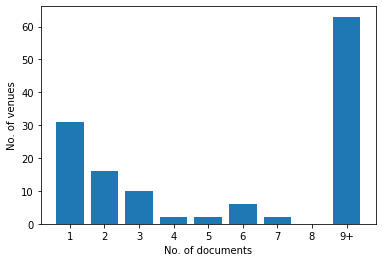
\includegraphics[width=.7\textwidth]{figures/evaluation/docs_per_venue.png}
    \caption{Number of documents per venue}
    \label{fig:docs_per_venue}
\end{figure}

Figure \ref{fig:docs_per_venue} shows the number of documents per venue. Almost half (48 \%) of the venues in our set are assigned to at least nine documents, whereas 23 \% are assigned to only one. These venues that are assigned to only one document are the professors of fields for which there weren't any popular venues in the repositories. Documents are usually only assigned one venue. This is always the case for publications, which are only be published in one place, but not necessarily for theses, which can have multiple advisors or referees. In our evaluation set, only 2 \% of the documents have more than one venue, and never more than two.

\subsubsection{Summary of the evaluation sets} \label{eval_datasets_summary}

After presenting each evaluation set individually, we now look at them as a whole, focusing on their coverage of repositories (table \ref{tab:eval_repo_coverage}) and fields (figure \ref{fig:eval_field_distribution}). We refer to them as the handwritten set, the \acrshort{ddc} set and the venue set for brevity.

The \acrshort{ddc} set covers by far the most documents of all repositories. As shown in table \ref{tab:eval_repo_coverage}, it covers 70 \% of the documents in all three repositories. depositonce is the repository worst represented in this evaluation set, with only 31 \% coverage. The handwritten set covers more than twice as many documents as the venue set. Contrary to the \acrshort{ddc} set, both these sets cover more of depositonce than of any other repository. This is remarkable given that depositonce is a much smaller repository than refubium.

\begin{table}[]
    \centering
    \begin{tabular}{|c|c|c|c|c|}
        \hline
        \textbf{Evaluation set} & \textbf{total} & \textbf{depositonce} & \textbf{edoc} & \textbf{refubium} \\ \hline \hline
        \textbf{Handwritten} & 24 \% & 29 \% & 23 \% & 22 \% \\ \hline
        \textbf{DDC} & 70 \% & 31 \% & 78 \% & 86 \% \\ \hline
        \textbf{Venues} & 11 \% & 16 \% & 14 \% & 8 \% \\ \hline
    \end{tabular}
    \caption{Repository coverage of the evaluation sets.}
    \label{tab:eval_repo_coverage}
\end{table}

Figure \ref{fig:eval_field_distribution} compares the coverage of the \acrshort{mag} fields by the evaluation sets, in percentages. The field percentages of an evaluation set results add up to 100 \%. The \acrshort{ddc} evaluation set is the most polarized of all. 18 \% of its documents belong to the field of \textit{Medicine}, and the fields \textit{Biology}, \textit{Physics} and \textit{Economics} each represent 13 \% of the evaluation set. Thus, 57 \% of the documents of the \acrshort{ddc} evaluation set belong to only four fields, out of 19.

The popularity of \textit{Medicine} in the \acrshort{ddc} set results of its large coverage of refubium (86 \%), which is the largest repository of the three and includes documents from Charité, the Medical University of Berlin. \textit{Economics} is a popular field both in \textit{refubium} and \textit{edoc}, as was discussed in chapter \ref{repo_analysis_subjects}. Furthermore, the \acrshort{ddc} evaluation set does not have any documents of the fields \textit{Materials science}, \textit{Business} and \textit{Environmental science}, as well as barely any belonging to \textit{Art} or \textit{Geography}. Therefore, there are three empty fields and two that are barely represented in this set.

The handwritten set is the most evenly distributed set regarding fields, and is the only one that covers all fields. The fields that stand out the most are \textit{Biology}, which accounts for 12 \% of the documents, followed by \textit{Medicine} and \textit{Physics}, both with 8 \% of the documents. Its worst represented fields are \textit{Business}, \textit{Environmental Science} and \textit{Art}, which are also among the least represented fields of the \acrshort{ddc} set.

The venue set is dominated by depositonce and edoc, which almost double refubium regarding repository coverage. This explains the two most popular fields, which differ from those in the other evaluation sets, as they do not appear often in refubium: \textit{Chemistry} accounts for 13 \% of the documents, and \textit{Computer science}, for 12 \%. On the other hand, this set doesn't have any documents for \textit{Art} and barely any for \textit{Philosophy}, \textit{History}, \textit{Geology}, \textit{Sociology}, \textit{Business} and \textit{Political Science}. These seven fields account for only 4.5 \% of the documents of this evaluation set.

\begin{figure}
    \centering
    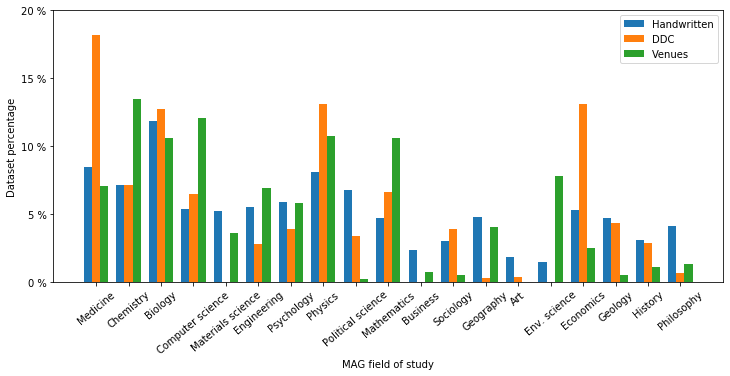
\includegraphics[width=\textwidth]{figures/evaluation/eval_field_distribution.png}
    \caption{Distribution of the evaluation set among the MAG fields of study.}
    \label{fig:eval_field_distribution}
\end{figure}

The natural sciences dominate all evaluation sets. It can be clearly seen in figure \ref{fig:eval_field_distribution}, where the bars to the left are much higher than those to the right. \textit{Medicine}, \textit{Biology} and \textit{Physics} appear more than 1,200 times in all three evaluation sets, mainly due to the \acrshort{ddc} evaluation set, which covers far more documents than the other two sets. On the other end of the spectrum, \textit{Art} and \textit{Business} are the only fields with less than 100 appearances in the evaluation sets. However, the average number of appearances per field exceeds 540 documents.
\subsection{Evaluation metrics} \label{eval_metrics}

In this section, we present evaluation metrics that are commonly used in the literature. Choosing the right metric is very important when measuring the performance of the model. Before doing so, one should first decide which aspects of the use case are the most relevant, as different metrics measure different things. For instance, a model can be highly accurate but output few subjects. Accuracy is more relevant than completeness for some use cases, and in others, it is the other way around.

In section \ref{eval_metrics_flat}, we discuss evaluation metrics that can be used with any set of subjects, whether they have a hierarchy or not. These metrics are binary: an assignment is either right or wrong, there is nothing in between. We then look at metrics that were designed specifically for hierarchical sets of subjects, in section \ref{eval_metrics_hierarchy}. These metrics take into account how far the guessed subjects are from the correct ones, e.g. by looking at their common ancestors in the hierarchy. Such metrics are better suited for hierarchies of subjects, as accuracies can be evaluated more precisely.

Finally, we look at precision-recall curves in section \ref{eval_metrics_curve}. This metric overcomes the issue of picking a threshold value for the assignment probabilities, which is a subjective decision and strongly impacts the performance of the model. For example, for a threshold of 80 \%, we assign all subjects to documents whose probability scores are at least 80 \%. This determines how many subjects are assigned, and affects the performance of the model in the metrics presented in the previous sections.

Once we have presented all these metrics, we pick the ones we find suitable for our approach in section \ref{eval_metrics_our}. We have chosen metrics that consider the incompleteness of our evaluation set, which includes only a few subjects per document, if any.

\subsubsection{Flat metrics} \label{eval_metrics_flat}

Flat evaluation metrics are those that don't consider the hierarchy of the subjects, or any relationship between subjects, for that matter. Each assignment is considered to be either right or wrong. There are two main types of flat metrics \cite{giraldo2015evaluation}:

\begin{enumerate}
    \item \textbf{label-based metrics}, which evaluate the performance for each label (i.e. subject, in our case), and
    \item \textbf{example-based metrics}, which evaluate the performance for each example, which in our case means a document in the evaluation set.
\end{enumerate}

We will look into both families of flat metrics, as well as some of their variations, in the following sections.

\paragraph{Label-based metrics} \mbox{}

The three most common label-based metrics for text classification are precision, recall and the F-score \cite{sebastianini2002machine}. They are all computed with the number of true positives (TP), false positives (FP), true negatives (TN) and false negatives (FN). In our case, a TP is a correctly assigned subject, whereas a FP is an incorrectly assigned subject. Analogously, a TN is a subject that was correctly discarded, and a FN is a subject that is not assigned, but should have been. Thus, \textit{true} and \textit{false} define if the decision has been right or wrong, and \textit{positive} and \textit{negative} express if the subject was assigned or not.

\textit{Precision} ($P$ in the formula below) describes how often assignments are correct. \cite{sebastianini2002machine} refers to precision as the \textit{degree of soundness} of an index. A low precision means that many of the assigned subjects are wrong, whereas a high precision means that few errors were made. It is important to note that this metric does not consider the number of assignments. For example, a model can have perfect precision (i.e. $P=1$) by only assigning one subject to a document. This method is inferior to another method that assigns thousands of subjects, with a lower precision of, say, $P=0.9$. Therefore, precision is usually evaluated together with recall.

$$ P = \frac{TP}{TP + FP} $$

\textit{Recall} ($R$ in the formula below) describes how many of the made assignments are correct, in contrast with how many correct assignments are missing. \cite{sebastianini2002machine} describes recall as the \textit{degree of soundness} of an index, which makes sense looking at the example above: it is not sound, given it has only made one assignment. Even if this single assignment is correct, many other correct assignments are missing.

$$ R = \frac{TP}{TP + FN} $$

Precision and recall are often combined, as they measure two important aspects of the assignments and complement each other very well. The \textit{F-score} combines precision and recall with a parameter $\beta$, which determines the relative importance of them \cite{medelyan2008domain}. $\beta$ is usually set to one, resulting in the harmonic mean of precision and recall, shown in the formula below.

$$ F_1 = 2 \frac{P \cdot R}{P + R} $$

\paragraph{Averaging methods} \mbox{}

The three metrics presented above can be computed in three different ways:

\begin{enumerate}
    \item \textbf{Micro-average}: all results are considered at the same time.
    \item \textbf{Macro-average}: results are grouped by subject.
    \item  \textbf{Sample-based average}: results are grouped by document.
\end{enumerate}

Macro-averaged metrics consider all assignments at once regardless of the subject or the document. The metric is computed once with all assignments. We illustrate this below with the formula for the macro-averaged precision.

$$ P_{macro} = \frac{1}{|S|} \sum_{s \in S} P_s  $$

Micro-averaged metrics, on the other hand, compute the metric for each subject separately, and then average over the results. Below we show the formula for the micro-averaged precision.

$$ P_{micro} = \frac{\sum_{s \in S} TP_s}{\sum_{s \in S} TP_s + FP_s}   $$

Each of these aggregation methods has its advantages and disadvantages: which metric or aggregation method is better depends on the application \cite{toepfer2020fusion}. For instance, the $F_1$-score does not consider TN, as its value is dominated by the number of TP \cite{gargiulo2019deep}. Therefore, smaller classes have little influence in the resulting score when micro-averaging. This is not an issue for use cases where the number of correct assignments matters more than having a consistent performance across labels. On the other hand, macro-averaged results give an equal weight to each class, and is better suited for cases where all subjects are equally important, regardless how often they are assigned to documents.

\paragraph{Example-based metrics} \mbox{}

Example-based metrics, as mentioned at the beginning of this section, evaluate examples of the evaluation set instead of labels. In our case, an example is a document in the evaluation set. Studies indicate that example-based metrics are better suited for multi-label settings, as they consider all subjects simultaneously \cite{giraldo2015evaluation}. Precision, recall and F-scores can also be computed regarding the intersection of the set of predicted subjects $\hat{Y}_d$ with the set of true subjects $Y_d$ \cite{gargiulo2019deep}. For instance, the \textit{example-based precision} ($P_{EB}$ in the formula below), estimates how many predicted labels are correct.

$$ P_{EB} = \frac{1}{|D|} \sum_{d \in D} \frac{|Y_d \cap \hat{Y}_d|}{|Y_d| + |\hat{Y}_d|} $$

\paragraph{Accuracy} \mbox{}

Accuracy does not depend on the micro- or macro-average, and is an alternative to precision and recall \cite{gargiulo2019deep}. However, it is not often used in text classification because the large denominator (the number of subjects) makes this metric insensitive to variations in the number of correct decisions \cite{sebastianini2002machine}. Another issue is that, given that in multi-label settings there are usually many more true negatives than true positives, making no assignments often yields the best accuracy. This does not happen with the F1-score.

$$ Acc = \frac{\sum_{s \in S} \frac{TP_s + TN_s}{TP_s + TN_s + FP_s + FN_s}}{|S|} $$

\subsubsection{Hierarchical metrics} \label{eval_metrics_hierarchy}

Hierarchical metrics are designed specifically for hierarchical sets of subjects. They take into account how far the guessed subjects are from the correct ones, e.g. by looking at their common ancestors in the hierarchy. For example, if a document is assigned the subject \textit{k-nearest neighbors}, which is a clustering algorithm, predicting the subject \textit{neural network} is closer than \textit{urban planning}, although both predictions are wrong. Hierarchical metrics aim to recognize the difference between both predictions, penalizing \textit{urban planning} more than \textit{neural network}.

These metrics assume that the assignments are consistent. If a subject is assigned to a document, all its ancestors in the hierarchy should also be assigned to the same document. In the case of \textit{k-nearest neighbors}, its parents would be \textit{clustering algorithms}, \textit{machine learning} and \textit{computer science}, for example. Precision, recall and F-scores can be adapted to hierarchical structures of subjects by considering the sets of predicted and true labels \cite{gargiulo2019deep}. In fact, they already do so in their example-based formulations, if the assignments are consistent with the hierarchy.

Common ancestors between predicted and true subjects increase the performance of the model in these metrics, as they are all included in the sets of subjects. However, adding all the ancestors can also lead to overestimating errors when the hierarchy has many levels. If assigned subjects have many ancestors, the sets of assigned and predicted subjects will be very large and may differ greatly, even if the predicted and assigned subjects are not so semantically different.

\cite{kosmopoulos2015evaluation} proposes several metrics that, instead of comparing complete sets of subjects, looks for the common ancestors of true and predicted subjects. The \acrfull{lca} of two nodes is the node that is furthest from the root, considering the common ancestors of the two nodes. As we don't know how to map the predicted subjects to the true ones, we consider all true subjects when looking for the \acrshort{lca} of a predicted subject. Thus, each predicted subject is compared to its most similar subject in the true set of subjects. The same is done the other way around, i.e. looking for the \acrshort{lca} for each true subject with the set of predicted subjects. Then we have again two sets of subjects, and the common metrics such as precision, recall and F-scores can be computed.

\subsubsection{Precision-recall curves} \label{eval_metrics_curve}

\acrfull{mlc} models usually output assignment probabilities for the subject, finally assigning those that are above a certain threshold. The choice of a threshold depends on what the assigned subjects are going to be used for. For instance, if one wants to relate documents to one another, a lower threshold will be picked, so that each document has more subjects, which results in more connections to other documents. On the other hand, if wrong predictions are not acceptable, like for example in the biomedical field, a higher threshold would be better.

Therefore, research on \acrshort{mlc} is usually evaluated with precision-recall curves \cite{wehrmann2018hierarchical}, which plot the trade-off between precision and recall for different threshold values (i.e. from zero to one). To enable the comparison between different curves, the area under the curve is measured. which results in a scalar that can be easily compared across methods. A higher area under the curve means that both the recall and the precision are high. Therefore, models with higher areas are considered better.

\subsubsection{Our metrics} \label{eval_metrics_our}

The researchers that use the metrics presented above use complete evaluation sets, where the subjects have been manually assigned to the documents. They are also noisy, given the lack of inter-indexer consistency \cite{csomai2007investigations}, but each document has multiple assigned subjects, which together describe their ``aboutness''. Our evaluation sets, as discussed in section \ref{eval_datasets_summary}, are sparse. They include only a few assignments per document, usually just one and sometimes none. We have to take this aspect into account when picking evaluation metrics.

Here we present the two metrics we use to evaluate the two approaches. The first one, called accuracy, checks if the correct subject is included among the top $n$ subjects output by a given model. The second metric, called \acrfull{lcas}, quantifies the \acrfull{lca} between the correct subject and the top $n$ subjects output by a model. The second metric is only used in the handwritten evaluation set, as the other two evaluation sets only consider fields, which don't have any ancestors.

\paragraph{Hit rate} \mbox{}

\textit{Hit rate} is an intuitive metric that measures how often the correct subject is within the top $n$ candidates output by a model as a percentage. We consider each assignment individually, checking if it is in the list of candidates or not. Then we divide the number of correct inclusions by the number of total checks. If a document has multiple assignments, each are considered independently.

For the \acrshort{ddc} and venue evaluation sets, where there are only 19 possible assignments, the number of candidates ranges from one to five. For the handwritten evaluation set, where there are 2,157 possible assignments, we consider 5, 10, 20, 30 and 50 candidates. Recall that the subject assignments of this dataset are not necessarily those that best represent their respective documents, and therefore are not expected to be on their top 5 or 10 candidates.
 
This metric is analogous to the one used in object recognition tasks in ImageNet \cite{russakovsky2015imagenet}, called \textit{error rate}, where they count misses instead of hits. Considering a variable number of candidates, they measure how often the correct assignments are not included. Thus, a lower error rate is better. In our case, where we count hits, a higher hit rate is better.

\paragraph{LCAS} \mbox{}

The \acrfull{lcas} is based on the evaluation metric proposed in \cite{kosmopoulos2015evaluation}, which quantifies the similarity of two subjects based on their \acrfull{lca}. \cite{kosmopoulos2015evaluation} concludes that a set-based version of the F1-score is the best metric for most use cases, but that pair-based metrics might be better for special cases. As stated above, our evaluation set is special because of its incompleteness. It contains one assignment per document, if any. Therefore, we adapt their metric to our case.

We define this metric by considering a \textit{correct subject}, which is the subject assigned to a document in the evaluation set, and a \textit{candidate subject}, which is the subject assigned to a document by a model. The candidate subject doesn't have to be correct, i.e. it is not always the same as the correct subject. As mentioned above, the \acrshort{lca} of two subjects is the subject that is furthest from the root, considering the common ancestors of the two subjects. We quantify the \acrshort{lca} by measuring the length of the path from the root (i.e. the fields) to the \acrshort{lca}.

Given that the depths of the paths from the fields to the subjects vary depending on the subject, we divide the length of the path to the \acrshort{lca} by the length of the path to the subject. This normalizes the \acrshort{lcas}, so larger paths are not overestimated. We also add one to all paths, which is the same as adding another node above the fields. We do this, so fields don't receive an \acrshort{lcas} of zero, as their actual path length is zero. Furthermore, adding one to all paths avoids divisions by zero if the correct subject is a field.

As correct and candidate subjects may have multiple common ancestors in the same hierarchy level, we always pick the ancestor for which the \acrshort{lcas} is highest. This evaluation metric, as the first one, is parameterized by the number of candidates. The formal definition of the \acrshort{lcas} can be seen below, where $Y$ is the correct subject, $X$ is the candidate subject and $LCA(X,Y)$ is their \acrshort{lca}. $P(S)$ is the path from the root to the subject $S$, and $|P(S)|$ denotes the length of that path.

$$ LCAS(X, Y) = \frac{|P(LCA(X, Y))|+1}{|P(Y)|+1}$$

\paragraph{Example of the LCAS} \mbox{}

\begin{figure}
    \centering
    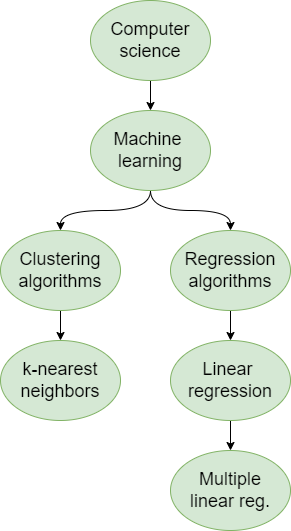
\includegraphics[width=.4\textwidth]{figures/evaluation/subject_hierarchy_example.png}
    \caption{Example of a subject hierarchy}
    \label{fig:subject_hierarchy_example}
\end{figure}

We illustrate the \acrshort{lcas} using the subject hierarchy shown in figure \ref{fig:subject_hierarchy_example}, which comprises subjects of the field \textit{Computer science}, with five hierarchy levels.

For correct subject \textit{Linear regression} and candidate subject \textit{Clustering algorithms}, the \acrshort{lca} would be \textit{Machine learning}. The path from the field \textit{Computer science} to the subject \textit{Linear regression} has length 3, as it passes through \textit{Machine learning} and \textit{Regression algorithms}. The length of the path to the \acrshort{lca} is 1. Thus, the \acrshort{lcas} for subject \textit{Linear regression} and candidate \textit{Clustering algorithms} is $\frac{1}{2}$. We show it in mathematical notation below, with each subject abbreviated to its initials for clarity.

$$ LCAS(CA, LR) = \frac{|P(LCA(CA, LR))|+1}{|P(LR)|+1} = \frac{|P(ML)|+1}{|P(LR)|+1} = \frac{2}{5} = \frac{1}{2} $$

If the correct subject were \textit{Multiple linear regression}, which descends from \textit{Linear regression}, the \acrshort{lcas} would be lower ($\frac{2}{5}$ instead of $\frac{1}{2}$). This is expected, as the descendant is further away from the \acrshort{lca}. On the other hand, if it were \textit{Machine learning}, which is an ancestor of the candidate, the \acrshort{lcas} would be $1$, which is its maximum value. This is also expected as the \acrshort{lca} is \textit{Machine learning} itself. The same \acrshort{lcas} would be achieved if the correct subject were \textit{Computer science}.

\begin{table}[]
    \centering
    \begin{tabular}{|c|c|}
        \hline
        \textbf{Correct subject} & \textbf{LCAS} \\ \hline\hline
        Computer science & 1 \\ \hline
        Machine learning & 1 \\ \hline
        Clustering algorithms & 1 \\ \hline
        k-nearest neighbors & 0.75 \\ \hline
        Regression algorithms & 0.67 \\ \hline
        Linear regression & 0.5 \\ \hline
        Multiple linear reg. & 0.4 \\ \hline
    \end{tabular}
    \caption{LCAS for several subjects where the candidate is \textit{Clustering algorithms}.}
    \label{tab:lcas_example}
\end{table}

In table \ref{tab:lcas_example}, we show several \acrshort{lcas} where \textit{Clustering algorithms} is the candidate subject. Here we can see that the \acrshort{lcas} decreases as we go deeper into the other subtree, and also that it is equal to one, the maximum value, when the correct subject is above the candidate subject in the hierarchy. Another interesting characteristic of the \acrshort{lcas} is that guesses that are further down in the hierarchy are rewarded. Thus, although the relative position of the subjects is the same, being close to a correct subject that is deeper in the hierarchy outputs a higher \acrshort{lcas}. For example, the \acrshort{lcas} of correct subject \textit{Linear regression} and candidate \textit{Regression algorithms} is $0.75$, whereas for correct subject \textit{Multiple linear regression} and candidate \textit{Linear regression}, the \acrshort{lcas} is $0.8$.

\subsection{Results of the unsupervised approach}

In this section, we assess the performance of the unsupervised approach with the evaluation sets. We first confirm the results of our qualitative assessment of the vector combination methods, which indicated that summing the vectors yields better results than averaging or concatenating them. The performance of the sum method on the venue and \acrshort{ddc} evaluation sets is considerably higher than that of the other two methods.

We then evaluate the performance of the sum method in the handwritten evaluation set. Its performance is lower than in the other evaluation sets, where only fields of study are considered. This is to be expected, given that there are 2,157 candidate subjects instead of 19, but it is still low.

We already discussed possible reasons for this difference in performance in section \ref{unsupervised_approach_conclusion}. The main challenge is the size of the dataset. The small amount of relationships that can be built between documents, and also between documents and venues, hinders the representations of the documents.

\subsubsection{Comparing the vector combination methods}

\begin{figure}
  \begin{subfigure}[t]{.45\textwidth}
    \centering
    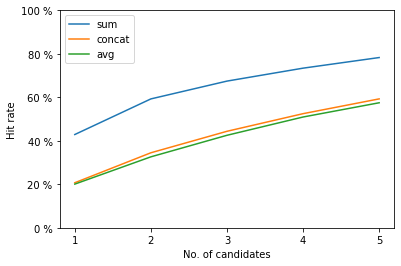
\includegraphics[width=\textwidth]{figures/unsupervised_approach/results/cosine_methods_ddc.png}
    \caption{DDC subjects}
    \label{fig:cosine_methods_ddc}
  \end{subfigure}
  \begin{subfigure}[t]{.45\textwidth}
    \centering
    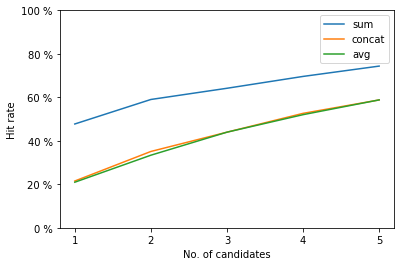
\includegraphics[width=\textwidth]{figures/unsupervised_approach/results/cosine_methods_venues.png}
    \caption{Venues}
    \label{fig:cosine_methods_venues}
  \end{subfigure}
  \caption{Hit rate of the three distance metrics in the evaluation sets.}
  \label{fig:combination_eval}
\end{figure}

We compare the three distance metrics on the two evaluation sets that consider fields, namely the \acrshort{ddc} and the venue evaluation sets. The hit rate of the combination methods is shown in figure \ref{fig:combination_eval}. The sum method outperforms the other two methods by a large margin in both datasets, the difference being usually over 20 \%. The other two methods behave similarly.

The sum method performs better for all considered numbers of candidates. It is also the most efficient, as all objects are represented by 100-dimensional vectors, as well as the only one that doesn't discard any information. The other two methods truncate word vectors, to match the sizes between the representations of documents and subjects.

\subsubsection{Results on the evaluation sets} \label{unsupervised_approach_results_eval}

\begin{figure}
  \begin{subfigure}[t]{.32\textwidth}
    \centering
    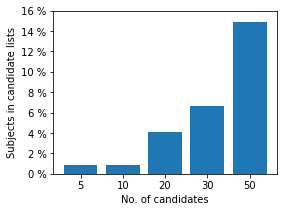
\includegraphics[width=\textwidth]{figures/unsupervised_approach/results/first_hw.png}
    \caption{Handwritten subjects}
    \label{fig:first_hw}
  \end{subfigure}
  \begin{subfigure}[t]{.32\textwidth}
    \centering
    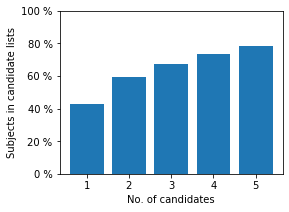
\includegraphics[width=\textwidth]{figures/unsupervised_approach/results/first_ddc.png}
    \caption{DDC subjects}
    \label{fig:first_ddc}
  \end{subfigure}
   \begin{subfigure}[t]{.32\textwidth}
    \centering
    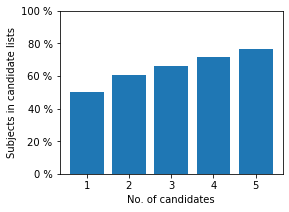
\includegraphics[width=\textwidth]{figures/unsupervised_approach/results/first_venue.png}
    \caption{Venues}
    \label{fig:first_venue}
  \end{subfigure}
  \caption{Hit rate of the unsupervised approach in the evaluation sets.}
  \label{fig:first_eval}
\end{figure}

Here we present the final results of the unsupervised approach, using the sum method as the distance metric. We have computed the distances between the documents and the subjects that descend from the five fields that are the closest to each document. We then store the 50 subjects that are the closest to each document. The hit rate of this approach on the evaluation set is depicted in figure \ref{fig:first_eval}. The hit rate on the \acrshort{ddc} and venue evaluation sets was already shown when comparing the different distance metrics.

The hit rate of this approach on the handwritten set is lower than in the other two datasets. Being accurate is much less likely in this set, as it has 2,157 options instead of 19, so the lower hit rate is to be expected. The hit rate of the model increases dramatically when more candidates are considered, reaching a maximum value of 15 \% when the 50 most similar subjects are considered. Recall that the subjects present in this evaluation set are not necessarily those that describe best the documents they are assigned to. They are merely those that appear in our subset of \acrshort{mag} subjects. Therefore, it is normal that the hit rate is so low when considering small numbers of candidates.

\begin{figure}
    \centering
    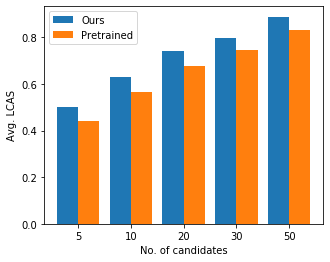
\includegraphics[width=.7\textwidth]{figures/unsupervised_approach/results/avg_lcas.png}
    \caption{Avg. LCAS of the unsupervised approach method, with and without pre-trained embeddings.}
    \label{fig:avg_lcas}
\end{figure}

\begin{figure}
    \centering
    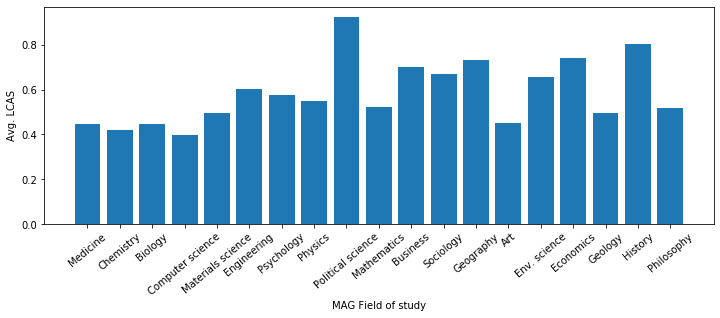
\includegraphics[width=\textwidth]{figures/unsupervised_approach/results/field_lcas.png}
    \caption{Avg. LCAS for each field using the unsupervised approach method and considering five candidates.}
    \label{fig:field_lcas}
\end{figure}

Regarding the \acrfull{lcas}, shown in figure \ref{fig:avg_lcas}, it steadily increases with the number of candidates, reaching a maximum average value of $0.89$. This value is very high, meaning that the guesses are close to the correct subjects in the subject hierarchy. We have also computed the average \acrshort{lcas} for each field, when considering five candidates. This is shown in figure \ref{fig:field_lcas}. \textit{Political Science} has a remarkably high value, over $0.9$, which results of averaging the \acrshort{lcas} of 898 assignments. Apparently, the model is accurately identifying the field.

On the other hand, \textit{Computer science} has a low average \acrshort{lcas} considering how popular the field is in our dataset. It may have to do with the fact that the subjects present in the handwritten set are not the top choices for the indexed documents and therefore do not appear in the top five candidates. When considering 50 candidates, \textit{Computer science} reaches an \acrshort{lcas} of $0.8$, and all other fields over $0.75$

\subsubsection{Using pre-trained embeddings} \label{unsupervised_approach_results_pretrained}

\begin{figure}
  \begin{subfigure}[t]{.32\textwidth}
    \centering
    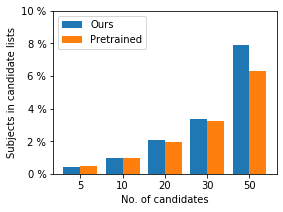
\includegraphics[width=\textwidth]{figures/unsupervised_approach/results/pretrained_hw.png}
    \caption{Handwritten subjects}
    \label{fig:pretrained_hw}
  \end{subfigure}
  \begin{subfigure}[t]{.32\textwidth}
    \centering
    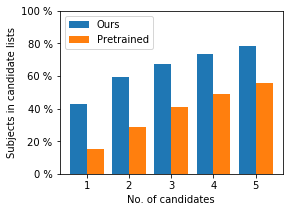
\includegraphics[width=\textwidth]{figures/unsupervised_approach/results/pretrained_ddc.png}
    \caption{DDC subjects}
    \label{fig:pretrained_ddc}
  \end{subfigure}
   \begin{subfigure}[t]{.32\textwidth}
    \centering
    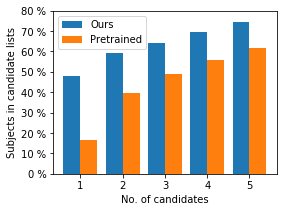
\includegraphics[width=\textwidth]{figures/unsupervised_approach/results/pretrained_venue.png}
    \caption{Venues}
    \label{fig:pretrained_venue}
  \end{subfigure}
  \caption{Hit rate of the unsupervised approach in the evaluation sets, with and without pre-trained embeddings.}
  \label{fig:pretrained_eval}
\end{figure}

Using pre-trained vector embeddings is common practice for \acrfull{nlp} tasks \cite{mikolov2017advances}. Such embeddings are trained on very large corpora and thus more accurately represent their corresponding words. Especially tasks on small datasets benefit from this transfer. However, technical datasets may not benefit as much from such pre-trained embeddings. They include words that are otherwise rare in non-scientific literature, and the style of writing is also different.

Here, we implement the same unsupervised approach, only changing the embeddings used to vectorize the texts. Instead of using the embeddings we have trained on our corpus, we use the pre-trained ones presented in section \ref{supervised_approach_embeddings}. Less than 3 \% of the words of our texts are not present in the file of pre-trained embeddings. If it were more, the lack of coverage would significantly hinder the performance of the method. This could still be the case, if the most distinctive words of each text are the ones missing.

Surprisingly, our own embeddings offer better results on the evaluation datasets, as shown in figure \ref{fig:pretrained_eval}. The method with our embeddings outperforms the one with the pre-trained embeddings on every dataset, for every number of candidates. Especially for the datasets regarding fields, the \acrshort{ddc} and venue datasets, the difference in hit rate is mostly around 30 to 50 \%. In the handwritten set, the difference is not so large, given that both models perform poorly.

This shows that our embeddings do a better job at representing the documents of the repositories. It is surprising that they are so much better, given the small size of our corpus. However, given how technical our corpus is, including fields both from the natural and the social sciences, it is to be expected that pre-trained embeddings don't work as well as in other use cases, where the data is similar to the one used to pre-train the embeddings.

The average \acrshort{lcas} of this method is depicted in figure \ref{fig:field_lcas} for several number of candidates. There it can be seen that using our own embeddings consistently improves the \acrshort{lcas} by $0.1$, which is a significant difference. Still, this method reaches an avg. \acrshort{lcas} of $0.8$ when considering 50 candidates.

\subsection{Results of the supervised approach} \label{results_supervised}

\begin{figure}
  \begin{subfigure}[t]{.5\textwidth}
    \centering
    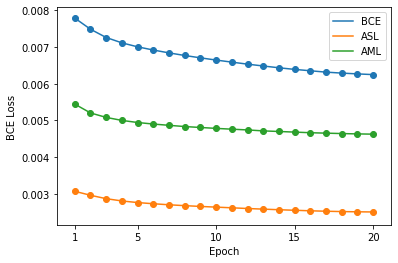
\includegraphics[width=\textwidth]{figures/supervised_approach/all_train_loss.png}
    \caption{Training loss}
    \label{fig:all_train_loss}
  \end{subfigure}
   \begin{subfigure}[t]{.5\textwidth}
    \centering
    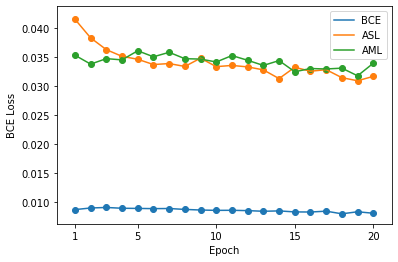
\includegraphics[width=\textwidth]{figures/supervised_approach/all_test_loss.png}
    \caption{Testing loss}
    \label{fig:all_test_loss}
  \end{subfigure}
  \caption{Test and training loss of the three final models.}
  \label{fig:all_train}
\end{figure}

\begin{figure}
  \begin{subfigure}[t]{.32\textwidth}
    \centering
    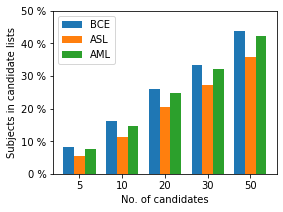
\includegraphics[width=\textwidth]{figures/supervised_approach/all_hw.png}
    \caption{Handwritten subjects}
    \label{fig:all_hw}
  \end{subfigure}
  \begin{subfigure}[t]{.32\textwidth}
    \centering
    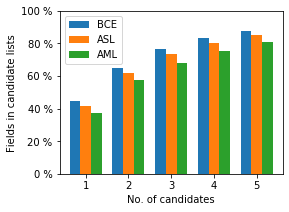
\includegraphics[width=\textwidth]{figures/supervised_approach/all_ddc.png}
    \caption{DDC subjects}
    \label{fig:all_ddc}
  \end{subfigure}
   \begin{subfigure}[t]{.32\textwidth}
    \centering
    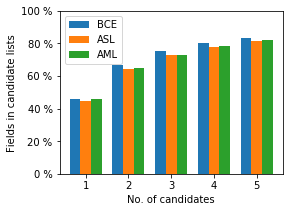
\includegraphics[width=\textwidth]{figures/supervised_approach/all_venue.png}
    \caption{Venues}
    \label{fig:all_venue}
  \end{subfigure}
  \caption{Hit rate of the three final models for the evaluation sets.}
  \label{fig:all_eval}
\end{figure}

Now we compare the three supervised models presented in section \ref{supervised_approach_models}, each with a different loss function: the \acrshort{bce} model, the \acrshort{asl} model and the \acrshort{aml} model. We use the best models that result from the experiments, presented in appendix \ref{supervised_approach_experiments}, and train them for an additional 20 epochs.

The testing loss of the \acrshort{bce} model is significantly lower, whereas the other two testing losses are similar, as shown in figure \ref{fig:all_train}. The training losses are very similar for all three models, differing in the thousandths. The training loss of the \acrshort{bce} model decreases the most out of the losses of the three models. On the other hand, the testing losses remained very steady for all three models. The \acrshort{asl} model seems to have benefitted the most from the additional training.

The \acrshort{bce} model yields the best hit rate on all three evaluation sets, as can be seen in figure \ref{fig:all_eval}, as well as the best \acrshort{lcas}, shown in figure \ref{fig:all_lcas}. The difference in hit rate to the other models is consistently around two percentage points throughout all numbers of candidates. The \acrshort{aml} model outperforms the \acrshort{asl} model on the handwritten evaluation set.  However, the \acrshort{asl} model has a better \acrshort{lcas}, meaning that its guesses are overall better than those of the \acrshort{aml} model. Furthermore, it performs better on the \acrshort{ddc} evaluation set. Still, both models don't perform as well as the \acrshort{bce} model. This could be because the model parameters and the training settings were optimized for that model, and the further extensions introduced by the other two models required other values for those parameters.

\begin{figure}
    \centering
    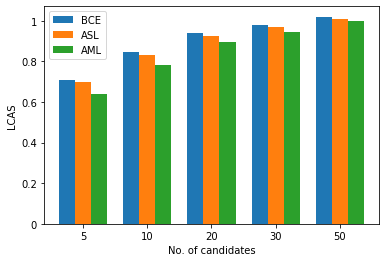
\includegraphics[width=.6\textwidth]{figures/evaluation/all_lcas.png}
    \caption{LCAS comparison of the three models.}
    \label{fig:all_lcas}
\end{figure}
\subsection{Comparison of the approaches} \label{results_final}

\begin{figure}
  \begin{subfigure}[t]{.32\textwidth}
    \centering
    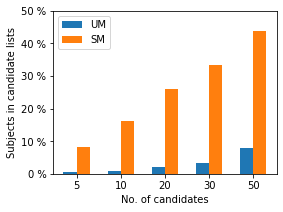
\includegraphics[width=\textwidth]{figures/supervised_approach/compare_hw.png}
    \caption{Handwritten subjects}
    \label{fig:compare_hw}
  \end{subfigure}
  \begin{subfigure}[t]{.32\textwidth}
    \centering
    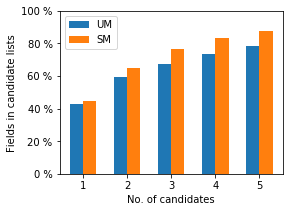
\includegraphics[width=\textwidth]{figures/supervised_approach/compare_ddc.png}
    \caption{DDC subjects}
    \label{fig:compare_ddc}
  \end{subfigure}
   \begin{subfigure}[t]{.32\textwidth}
    \centering
    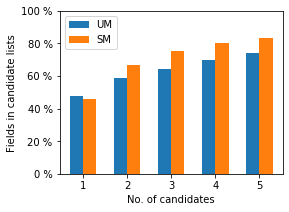
\includegraphics[width=\textwidth]{figures/supervised_approach/compare_venue.png}
    \caption{Venues}
    \label{fig:compare_venue}
  \end{subfigure}
  \caption{Hit rate of the approaches for the evaluation sets.}
  \label{fig:compare_eval}
\end{figure}

\begin{figure}
    \centering
    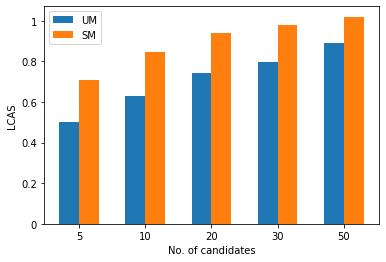
\includegraphics[width=.6\textwidth]{figures/evaluation/compare_lcas.png}
    \caption{LCAS comparison of the approaches.}
    \label{fig:compare_lcas}
\end{figure}

In this section, we compare the unsupervised approach with the best performing supervised model, i.e. the \acrshort{bce} model. We refer to them as \acrfull{um} and \acrfull{sm}, respectively. The \acrshort{sm} outperforms the \acrshort{um} in all evaluation sets, as shown in figure \ref{fig:compare_eval}. The \acrshort{sm} is better at identifying fields than the \acrshort{um}. It performs consistently better on the \acrshort{ddc} and venue evaluation sets. However, the difference in hit rate is the largest for the handwritten set.

Only in the venue set for one candidate does the \acrshort{um} perform better, by a margin of 2 \%. For all other number of candidates, the \acrshort{sm} performs better, by a margin from 8 to 11 \%. The differences on the \acrshort{ddc} set are similar. The difference in performance when identifying all 2,157 subjects is much larger, also in favor of the \acrshort{sm}. The difference between them goes from 8 \% when 5 candidates are considered, to 36 \% for 50 candidates.

The superiority of the \acrshort{sm} on the handwritten set is also confirmed by the \acrshort{lcas}, shown in figure \ref{fig:compare_lcas}. Given the large difference in hit rate between the models, this result is to be expected. However, that the \acrshort{lcas} difference is smaller than the difference in hit rate indicates that the guesses of the \acrshort{um} are close to the correct subjects. This hypothesis is also supported by the high hit rate of the \acrshort{um} when identifying fields in the other two evaluation sets.
\subsection{Impact of document length on hit rate} \label{results_length}

\begin{figure}
  \begin{subfigure}[t]{.32\textwidth}
    \centering
    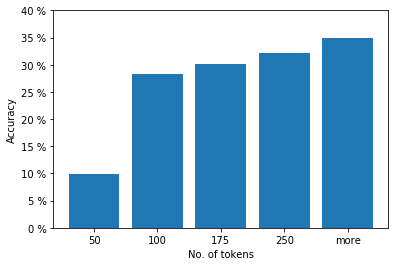
\includegraphics[width=\textwidth]{figures/supervised_approach/sm_hw_length.png}
    \caption{Handwritten subjects}
    \label{fig:sm_hw_length}
  \end{subfigure}
  \begin{subfigure}[t]{.32\textwidth}
    \centering
    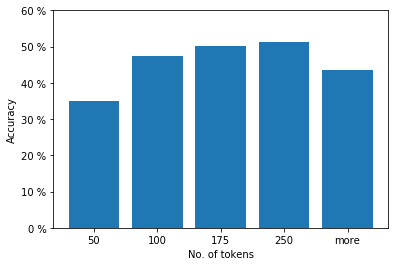
\includegraphics[width=\textwidth]{figures/supervised_approach/sm_ddc_length.png}
    \caption{DDC subjects}
    \label{fig:sm_ddc_length}
  \end{subfigure}
   \begin{subfigure}[t]{.32\textwidth}
    \centering
    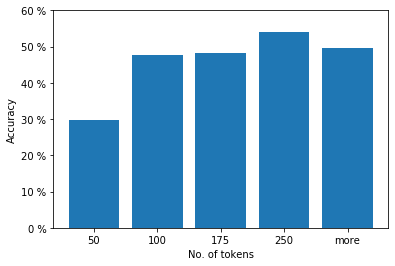
\includegraphics[width=\textwidth]{figures/supervised_approach/sm_venue_length.png}
    \caption{Venues}
    \label{fig:sm_venue_length}
  \end{subfigure}
  \caption{Hit rate of the approaches for the evaluation sets, grouped by representation length. We consider 20 candidates for the handwritten set, and 1 for the two others.}
  \label{fig:sm_eval_length}
\end{figure}

In this section, we analyze how the length of the documents affects the hit rate of the \acrshort{sm}, our most accurate model. We already showed the representation lengths of the documents after mapping their tokens to the pre-trained vectors in figure \ref{fig:sm_doc_length}. Over 8,000 documents were represented by less than 50 word vectors, and over 6,000 documents have less than 100 vectors. Here, we compute the accuracies on the evaluation set for each length group.

Figure \ref{fig:sm_eval_length} shows the accuracies of the \acrshort{sm} on the evaluation sets for the different length groups. In contrast to the other figures displaying model hit rate, here the number of candidates is fixed. Instead of considering all documents at once, we compute the hit rate for each length group. The hit rate for documents with less than 50 tokens is significantly worse than for documents with more than 50 tokens. The difference in the \acrshort{ddc} and venue sets between the shortest documents and the rest ranges between 15 and 20 \% for the most part. For the handwritten set, the difference is even larger: between 20 and 25 \%. This shows that the model's hit rate is considerably hindered when the representation of the document comprises less than 50 vectors.

The hit rate of the model steadily increases with longer representations, but at a much lower rate. Recall that representations with more than 250 tokens are truncated; only the first 250 tokens are fed to the model. We thus conclude that the representation length does impact the hit rate of the model. Documents represented with less than 50 documents are especially challenging for the model. If we discarded these documents, the hit rate of the model would increase by at least 20 \% on all evaluation sets.
